\chapter{Experiments}
\label{ch:method}
\section{Implementation}
In the training phase, the stratified sampling approach was employed, where 10\% of the data was allocated for testing purposes and the remaining 90\% for training. The data was randomly split using the Scikit-learn package\cite{b31}. This strategy was selected to maintain consistent label proportions in the test and training sets. By doing so, we aimed to prevent the risk of insufficient genuine samples that could occur with random sampling.\\

The 5-fold cross-validation was implemented with Scikit-learn to train the SVM and XGBoost and determine the best-performing model for final evaluation. Fine-tuning of PLMs was conducted using checkpoints provided by Hugging Face, using the AdamW optimizer\cite{b32} and cross-entropy loss. The learning rate was set to 2e-5, and training was carried out for 20 epochs. HAN was trained for the same number of epochs with its default settings\cite{b33}. The training procedure was repeated five times with different random seeds, and checkpoints of models were selected for final evaluation based on the highest validation F1-score\cite{b34}. HAN was trained on the Tesla T4, while all other PLMs were trained on the RTX A5000.
\begin{figure}
  \centering
  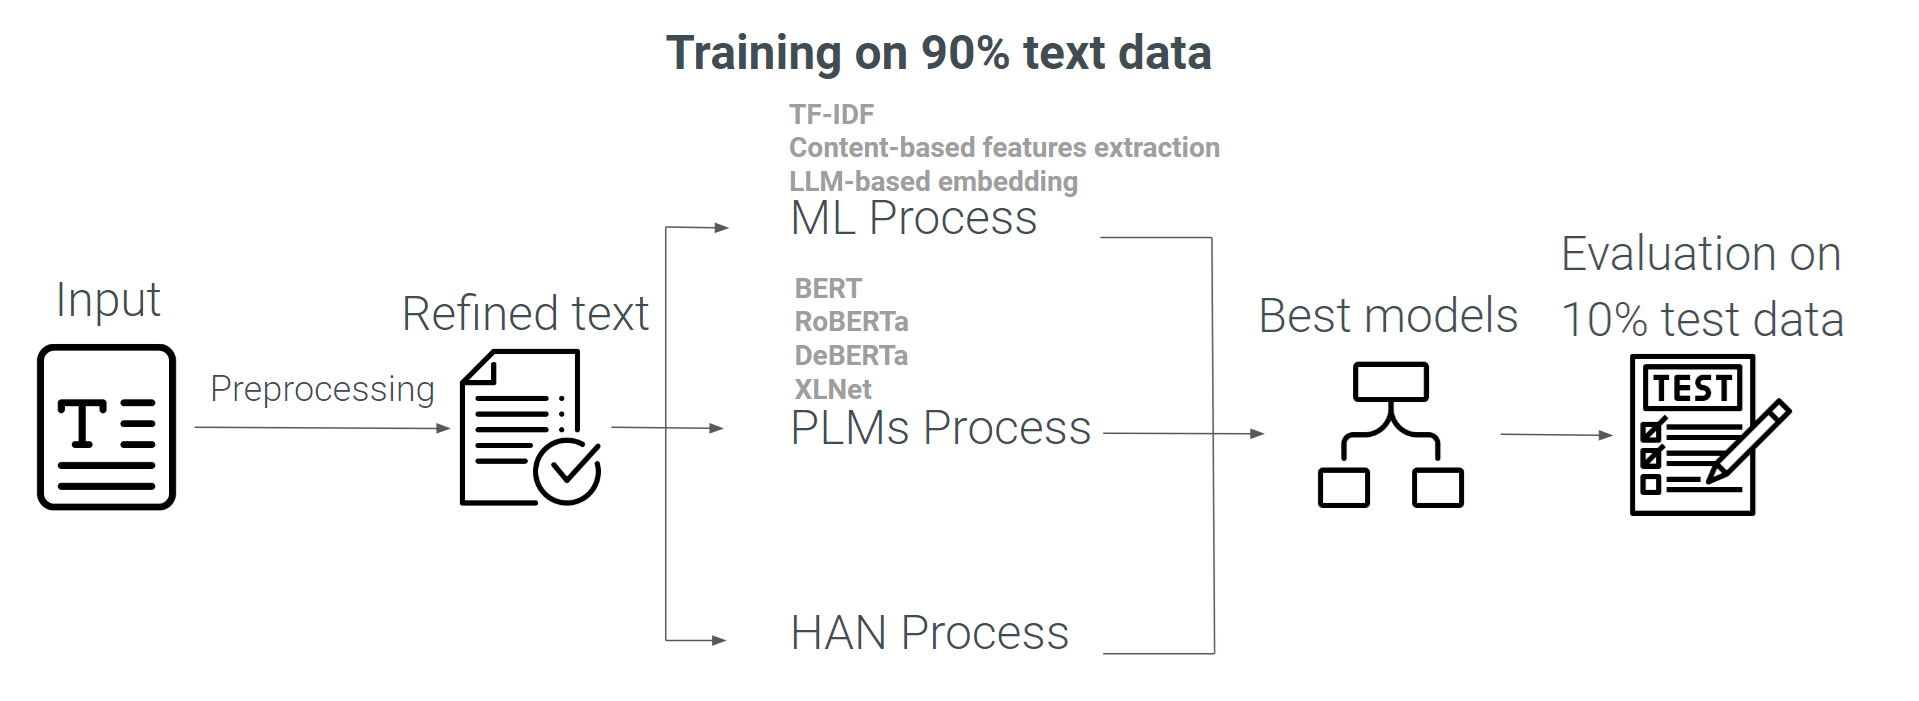
\includegraphics[width=1\columnwidth]{img/training2.png}
  \caption{The implementation workflow for the experiments. } 
  \vspace{-0.4cm}
  \label{fig:training}
\end{figure}
\\
The Fig. \ref{fig:training} illustrates the implementation workflow for the experiments. The model used the processed text as input and outputted a binary classification result (0 or 1), representing the categories of "genuine" or "fake". Finally, common metrics were calculated to evaluate the performance of the models.

\section{Configuration}
This study summarized the detailed information about implementation. For TF-IDF feature generations, the configurations illustrated in Table \ref{tab:TFIDF_detail} were used. Regarding implementations of the BERT series, the parameter settings were summarized as Table \ref{tab:BERT_detail} present. Acknowledging that changing parameter settings can result in diverse outcomes, we followed the configuration of the previous studies\cite{b5,b31,b33} to fine-tune the pre-trained models used in the experiments. This approach ensures that our models are optimized for performance and reliability across different scenarios and datasets.

\begin{table}
    \centering
    \caption{Parameter settings of TF-IDF features extractor.}
    \label{tab:TFIDF_detail}
\begin{tabular}{|c|c|}
\hline
Parameter     & Configuration \\ \hline
Stop\_words   & None          \\
Ngram\_range  & (1, 1)        \\
Min\_df       & 1             \\
Max\_features & None          \\ \hline
\end{tabular}
\end{table}


\begin{table}
    \centering
    \caption{Parameter settings for fine-tuning pretrained language models (PLMs)}
    \label{tab:BERT_detail}
\begin{tabular}{|c|cccc|}
\hline
Parameter      & BERT     & RoBERTa  & DeBERTa  & XLNet    \\ \hline
Max\_length    & 256      & 256      & 256      & 256      \\
Batch\_size    & 64       & 64       & 32       & 64       \\
Learning\_rate & 2e-5     & 2e-5     & 2e-5     & 2e-5     \\
Epochs         & 20       & 20       & 20       & 20       \\
Val\_metric    & F1-score & F1-score & F1-score & F1-score \\ \hline
\end{tabular}
\end{table}

\section{Evaluation metrics}
The concept of a confusion matrix is commonly used in classification tasks to evaluate the performance of machine learning models. It provides a detailed breakdown of the predictions made by the model compared to the actual ground truth. The confusion matrix consists of four primary elements:
\begin{itemize}
    \item True Positive (TP): These are the cases where the model correctly predicts the positive class.
    \item False Positive (FP): These are the cases where the model incorrectly predicts the positive class (i.e., predicts positive when the actual class is negative).
    \item True Negative (TN): These are the cases where the model correctly predicts the negative class.
    \item False Negative (FN): These are the cases where the model incorrectly predicts the negative class (i.e., predicts negative when the actual class is positive).
\end{itemize}

In evaluating the performance of classification models, several vital metrics such as accuracy, precision, recall, F1-score, and Area Under the Curve (AUC) are commonly used to provide a comprehensive assessment based on the confusion matrix. 

Accuracy is one of the famous metrics for classification tasks. This metric evaluates how often the model makes correct predictions by comparing the number of correctly predicted observations to the total number of observations. Accuracy can be calculated via the following formula:
\begin{equation}
    Accuracy = \frac{TP+TN}{TP+TN+FP+FN}
\end{equation}

% \subsection{Precision and Recall}
Precision is the ratio of correctly predicted positive observations to the total predicted positive observations, also known as the positive predictive value. Recall, or sensitivity, measures the ratio of correctly predicted positive observations to all actual positives. Precision and recall are calculated using:
\begin{equation}
    Precision = \frac{TP}{TP+FP}
\end{equation}
\begin{equation}
    Recall = \frac{TP}{TP+FN}
\end{equation}

% \subsection{F1-score}
F1-score balances precision and recall by taking their harmonic mean. It is beneficial when we need to consider both false positives and false negatives for a more accurate evaluation of model performance. This metric is particularly helpful when dealing with imbalanced datasets, providing a more accurate evaluation of the model's performance. The formula for F1-score is:
\begin{equation}
    F1\text{-}score = 2×\frac{Precision×Recall}{Precision+Recall}
\end{equation}

% \subsection{AUC}
The Area Under the Curve (AUC) measures the model's capability to distinguish between classes and is used as the summary of a receiver operating characteristic (ROC) curve. The ROC curve displays the model's determining ability as the discrimination threshold changes. A higher AUC value indicates a better ability of the model to distinguish between positive and negative instances correctly.

\section{Experimental results}
Model performances were evaluated using well-known metrics: accuracy, precision, recall, F1-score, and AUC. The results presented in Table \ref{tab:results} compare the proposed method with other approaches, including traditional machine learning algorithms, attention-based deep learning networks like HAN, pre-trained networks, and state-of-the-art LLMs. In addition, both the fuzzy rank-based method and soft voting method combine the RoBERTa, DeBERTa, and XLNet models.
\begin{table}[]
    \caption{ Comparison of the performance of different models for test data using various evaluation metrics includes accuracy, precision, recall, F1-score, and AUC.}
    \label{tab:results}
    \centering
\begin{tabular}{lccccc}
\hline
Model                   & Accuracy & Precision & Recall  & F1-score & AUC     \\ \hline
TF-IDF + SVM            & 89.08\%  & 91.46\%   & 95.34\% & 93.36\%  & 92.02\% \\
Engineered features + XGBoost        & 82.59\%  & 83.88\%   & 97.03\% & 89.98\%  & 78.95\% \\
HAN                     & 90.78\%  & 94.09\%   & 94.49\% & 94.29\%  & 93.09\% \\
BERT                    & 91.13\%  & 93.75\%   & 95.34\% & 94.54\%  & 96.31\% \\
RoBERTa                 & 91.81\%  & 93.44\%   & 96.61\% & 95.00\%  & 96.59\% \\
DeBERTa                 & 91.81\%  & 94.17\%   & 95.76\% & 94.96\%  & 95.75\% \\
XLNet                   & 92.83\%  & 94.24\%   & 97.03\% & 95.62\%  & 96.12\% \\
Ada-002 + SVM     & 92.83\%  & 93.52\%   & \textbf{97.88\%} & 95.65\%  & 94.88\% \\
Gemini + SVM  & 91.47\%  & 92.71\%   & 97.03\% & 94.82\%  & 93.27\% \\
GPT-4                   & 82.25\%  & 91.82\%   & 85.59\% & 88.60\%  & N/A     \\
Soft voting             & 93.17\%  & 94.63\%   & 97.03\% & 95.82\%  & 97.14\% \\
Soft voting with features       & 92.49\%  & 93.15\%   & \textbf{97.88\%} & 95.45\%  & 96.52\% \\
Fuzzy rank-based method & \textbf{93.52\%}  & \textbf{94.65\%}   & 97.46\% & \textbf{96.03\%}  & \textbf{97.15\%}     \\ \hline
\end{tabular}
\end{table}
\subsection{TF-IDF with SVM}
TF-IDF with SVM achieved an accuracy of 89.08\%, precision of 91.46\%, recall of 95.34\%, F1-score of 93.36\%, and AUC of 92.02\%. However, it is crucial to acknowledge that the performance of TF-IDF with SVM can be constrained when dealing with complex text data that need a deeper understanding of contextual data relationships. While these metrics show acceptable performance, they are still beaten by attention-based deep models like the HAN and BERT series in the experiments.

\subsection{Engineered features with XGBoost}
The use of sectarian words, the strength of quoted sources/attribution, and linguistic features provided a certain degree of accuracy in classifying long COVID-related fake news. However, due to differences in the dataset, our study lacked the inconsistency score feature used in the original methodology. Therefore, the performance of this approach in the experiments was lower than other methods. Specifically, except for recall, all other metrics were below the baseline. The experiment results indicate that while these content-based features contribute to the classification task, the absence of the inconsistency score limited the overall usefulness.
Additionally, this aligns with our prior data analysis, particularly the sentiment analysis. In section 3.4.2, the sentiment analysis showed that genuine and fake articles overlap in neutral sentiment and subjectivity categories, suggesting that these textual features alone are insufficient for accurate classification. The similar sentiment distribution across genuine and fake texts may contribute to the limitations observed in the content-based feature approach.

\subsection{HAN}
The HAN model achieved an accuracy of 90.78\%, precision of 94.09\%, recall of 94.49\%, F1-score of 94.29\%, and an AUC of 93.09\% in the experiment. This demonstrated that HAN performed well in the text classification task, maintaining reasonable recall and F1-score while achieving high accuracy and precision. Comparing HAN with TF-IDF and BERT, we can observe that HAN outperforms TF-IDF in terms of accuracy (90.78\% vs. 89.08\%), F1-score(94.29\% vs. 93.36\%), and AUC (93.09\% vs. 92.02\%), indicating its superior performance in the study. However, BERT achieved slightly higher accuracy (91.13\%) and AUC (96.31\%) compared to HAN.
\subsection{BERT series}
With its self-attention mechanism, BERT achieved a notable performance better than TF-IDF in the study, showing the advantages of BERT's self-attention mechanism in capturing complex patterns in the text data. It achieved an accuracy of 91.13\%, precision of 93.75\%, recall of 95.34\%, F1-score of 94.54\%, and AUC of 96.31\%. Another interesting observation in the experiments is that extensions of BERT, such as RoBERTa, DeBERTa, and XLNet, consistently outperformed the original BERT model. This phenomenon indicates the usefulness of their individual improvement strategies. Among the BERT series, XLNet stands out as the top performer.
\subsection{LLMs}
Gemini and text-embedding-ada-002, based on the advancements of LLMs, converted textual data into high-dimension embedding vectors and achieved F1-score of 94.82\% and 95.65\%, respectively. The text-embedding-ada-002 had a precision of 93.52\%, recall of 97.88\%, accuracy of 92.83\%, and AUC of 94.88\%, exhibiting its ability to distinguish between genuine and fake news effectively. Conversely, GPT-4, which was directly used for text classification, had an accuracy of 82.25\%, indicating that its performance could have been more competitive than other models in the experiment. However, the performance was still acceptable even without training and fine-tuning. Due to the use of the GPT-4 API, it was not possible to properly obtain the model's probabilities for predicting fake and genuine labels, making the calculation of the AUC infeasible.
\subsection{Ensemble methods}
Last but not least, the ensemble methods, including soft voting and the fuzzy rank-based method, demonstrated their effectiveness by achieving F1-score of 95.82\% and 96.03\% in the experiments, respectively. These results outperformed individual models like conventional TF-IDF and state-of-the-art LLM, emphasizing the power of combining information from multiple models for enhanced final decision-making in text classification tasks. Especially the fuzzy method achieved impressive results on the test set, with an accuracy of 93.52\%, precision of 94.65\%, F1-score of 96.03\%, and AUC of 97.15\%, presenting the highest performance among all methods estimated. Fig. \ref{fig:confusion matrix} shows the confusion matrix with the top 4 F1-score in the experiment.
\begin{figure}
    \centering
    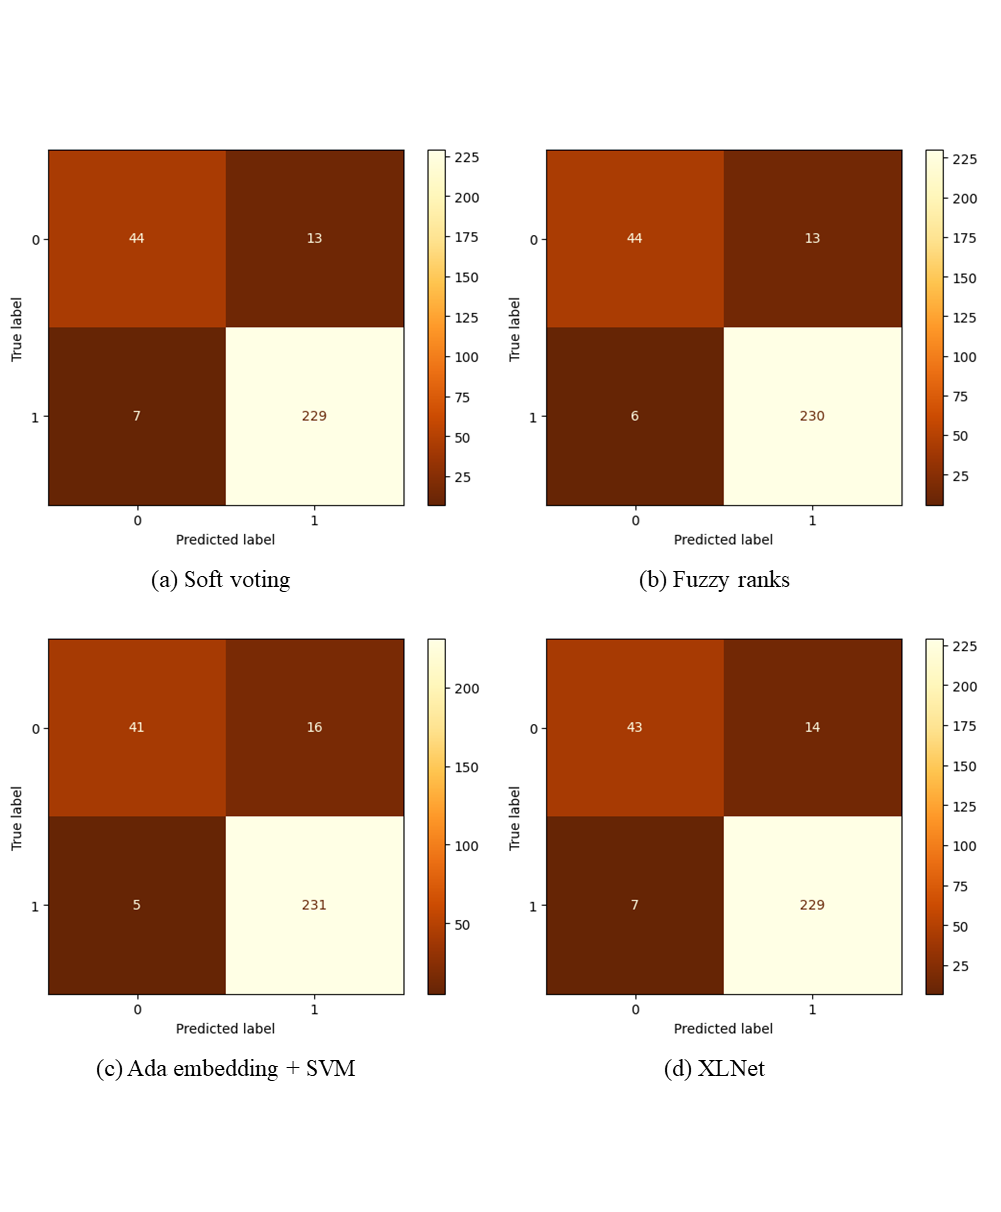
\includegraphics[width=1\linewidth]{img/CM4.png}
    \caption{Confusion matrix of (a) soft voting, (b) fuzzy rank-based method, (c) Ada embedding method and (d)XLNet on the held-out test dataset.}
    \label{fig:confusion matrix}
\end{figure}

On the other hand, despite attempting to enhance the classification ability by incorporating sectarian words, the strength of quoted sources/attribution, and linguistic features with soft voting probabilities, the experimental results indicated otherwise. Except for a slight improvement in recall, other metrics showed a minor decline. In contrast, the fuzzy rank-based ensemble method, which combines predictions from multiple models, demonstrated superior performance.
The possible explanation for this outcome is that different attention-based models already include information similar to the content-based features. Therefore, the absence of the inconsistency score introduced noise, adversely affecting the model's performance. This suggests that while content-based features are valuable, their effectiveness is diminished when the attention-based models already capture similar information.





\section{Real case inference}

Table \ref{tab:real case} is the actual case of using the fuzzy method to detect fake and genuine news that was not included in the test set. We used four isolated samples, two genuine and two fake, varying in short and long length. The result shows that our method accurately detected the genuineness of the content regardless of its length, revealing its robustness across different text lengths.


\begin{table}[]
    \caption{Real case inference using fuzzy rank ensemble method.}
    \label{tab:real case}
    \centering
\begin{tabular}{|l|c|c|c|}
\hline
\rowcolor[HTML]{31394D} 
{\color[HTML]{FFFFFF} Content / Mainly claim}                                                                                                                                                                                                                                                                                                                                                                                                                                                                                                                                                                                                                                                        & \multicolumn{1}{l|}{\cellcolor[HTML]{31394D}{\color[HTML]{FFFFFF} Length}} & \multicolumn{1}{l|}{\cellcolor[HTML]{31394D}{\color[HTML]{FFFFFF} Prediction}} & \multicolumn{1}{l|}{\cellcolor[HTML]{31394D}{\color[HTML]{FFFFFF} Ground truth}} \\ \hline
\begin{tabular}[c]{@{}l@{}}A German study has revealed long COVID is linked\\  to the vaccine.\end{tabular}                                                                                                                                                                                                                                                                                                                                                                                                                                                                                                                                                                                          & 15                                                                         & fake                                                                           & fake                                                                             \\ \hline
\begin{tabular}[c]{@{}l@{}}Covid vaccination before infection strongly linked to\\  reduced risk of developing long covid\end{tabular}                                                                                                                                                                                                                                                                                                                                                                                                                                                                                                                                                               & 15                                                                         & genuine                                                                        & genuine                                                                          \\ \hline
\begin{tabular}[c]{@{}l@{}}Long COVID's causes and risk factors remain a subject\\  of ongoing research, with potential factors including\\  reactivation of SARS-CoV-2 particles, overactive \\ immune responses, and the development of \\ autoantibodies attacking organs. Certain groups, such as\\  those with severe COVID-19 history, underlying health\\  conditions, or lacking vaccination, are at higher risk, \\ alongside other factors like sex, age, initial immune\\  response, and viral variants. Health inequities may\\  also contribute, especially affecting racial or ethnic \\ minority groups and individuals with disabilities.\end{tabular}                               & 367                                                                        & genuine                                                                        & genuine                                                                          \\ \hline
\begin{tabular}[c]{@{}l@{}}While Omicron's subvariants find new ways to \\ evade vaccines and destabilize immune systems, \\ another pandemic has overwhelmed offcials who \\ are supposed to be in charge of public health. \\ In any case, COVID, a novel virus that can wreak \\ havoc with vital organs in the body, continues \\ to evolve at a furious pace. In response officials have \\ largely abandoned any coherent response, including \\ masking, testing, tracing and even basic data collection.\\  Yes, the people have been abandoned. So don't expect \\ "normal" to return to your hospital, your airport, your \\ nation, your community or your life anytime soon.\end{tabular} & 469                                                                        & fake                                                                           & fake                                                                             \\ \hline
\end{tabular}
\end{table}